\documentclass[]{report}
\usepackage[hmargin=1.25in,vmargin=1in]{geometry} %调整页边距
% \usepackage[inner=1in,outer=1.25in]{geometry} %书籍左右不等宽排版
\usepackage[utf8]{inputenc}
\usepackage[]{ctex} %据说可以直接调用诸如 \kaishu \fangsong \heiti 的命令修改字体
\usepackage[svgnames]{xcolor} % Using colors
% \usepackage{background} % To include background images
\usepackage{fancyhdr} % Needed to define custom headers/footers
\usepackage[]{xeCJK}
\setCJKmainfont[BoldFont = STHeiti, ItalicFont = STKaiti]{Songti SC Light} %中文主字体
\setCJKsansfont[BoldFont = Weibei SC, ItalicFont = HanziPen SC]{Xingkai SC Light} %中文无衬线字体
\setCJKmonofont[BoldFont = Libian SC, ItalicFont = STFangsong]{Yuanti SC Light} %中文等宽字体
\setmainfont{Times New Roman} %\rmfamily
\setsansfont[ItalicFont = American Typewriter]{Comic Sans MS} %\sffamily
\setmonofont{Courier} %\ttfamily
\newfontfamily\monaco{Courier} % 用于代码段字体设置
\usepackage{titlesec}
\titleformat{\chapter}{\centering\huge\bfseries}{第~\thechapter~次作业}{1em}{}
\titleformat{\section}{\Large\bfseries}{第~\thesection~题}{1em}{}
\renewcommand{\thesubsection}{(\alph{subsection})}
\usepackage{lipsum} %填充文本

\usepackage{ulem} %解决下划线、删除线之类的
\usepackage{listings}
\lstset{
language=Matlab,
keywords={break,case,catch,continue,else,elseif,end,for,function,
global,if,otherwise,persistent,return,switch,try,while},
numberstyle = \monaco,
basicstyle = \monaco,
keywordstyle = \color{blue}\bfseries,
commentstyle=\color[HTML]{006400},
tabsize = 4,
backgroundcolor=\color[HTML]{F5F5F5},
emph = {cos, sin, tan, tanh, log, exp, abs, linspace, ones, zeros, plot, semilogy, legend, loglog, polyfit, polyval},emphstyle=\color[HTML]{8B008B}
}

\makeatletter
\newif\if@restonecol
\makeatother
\let\algorithm\relax
\let\endalgorithm\relax
\usepackage[linesnumbered,ruled,vlined]{algorithm2e}%[ruled,vlined]{
\usepackage{algpseudocode}
\usepackage{amsmath}
\renewcommand{\algorithmicrequire}{\textbf{Input:}}  % Use Input in the format of Algorithm
\renewcommand{\algorithmicensure}{\textbf{Output:}} % Use Output in the format of Algorithm

\usepackage{amsmath} %数学公式问题
\usepackage{amsthm} %公式环境,如proof
\usepackage{booktabs} %三线表
\newcommand{\tabincell}[2]{\begin{tabular}{@{}#1@{}}#2\end{tabular}} %解决单元格内部换行的问题
% 比如这个 Beijing & 0,5 & 1,6 & 2,7 & 3,8 & 4,9 & The number changes every 3 months \\
% 改成这个 \tabincell{l}{Beijing}& \tabincell{c}{0,5}& \tabincell{c}{1,6}& \tabincell{c}{2,7}& \tabincell{c}{3,8}& \tabincell{c}{4,9}& \tabincell{c}{The number changes \\ every 3 months} \\
% 一个单元格过长,整行都需要修改
% 可以配合 \resizebox*{h-width}{v-width}{contents, e.g.tabular} 使用

\usepackage{mathrsfs} %在公式里面使用那个最花的字体
\usepackage{amssymb} %公式里面用空心黑体和旧式字体
\usepackage{amssymb} %AMS符号
\usepackage{amsthm} %AMS定理环境

\usepackage{markdown} %使用markdown语法,在编译时需要打开 shell-escape 标记,即 $ xelatex --shell-escape example.tex
\markdownSetup{hashEnumerators = true} %允许使用 #. 的方式编写有序列表
\markdownSetup{inlineFootnotes = true} %允许使用脚注形式的超链接,调用语法为 [anchor](uri), ^[footnote], <uri>
\markdownSetup{fencedCode = true} %以反引号和缩进来插入代码段,相当于 verbatim
\markdownSetup{
  pipeTables = true
} %支持表格的用法 (图片已经在markdown包里面支持了)
% \usepackage{booktabs} %解决三线表的线条粗细问题

\usepackage{graphicx} %插入图片
\usepackage{pdfpages} %插入PDF文件
\usepackage{makeidx}

\usepackage{tikz} %带圈字符
\usepackage{etoolbox} %带圈字符 (提供robustify)
\usepackage{enumitem}
\newcommand*{\circled}[1]{\lower.7ex\hbox{\tikz\draw (0pt, 0pt)%
    circle (.5em) node {\makebox[1em][c]{\small #1}};}} %新定义命令:带圈字符
\robustify{\circled}
% \usepackage{enumerate} %有序列表

\usepackage{hyperref} %超链接
% \usepackage[hidelinks]{hyperref} %隐藏超链接的红框
\markdownSetup{
  inlineFootnotes = true,
  renderers = {
    link = {\href{#3}{#1}},
  }
} % markdown块中使用直接点进去的超链接
% \setlist[enumerate,1]{label=(\arabic*).,font=\textup,leftmargin=7mm,labelsep=1.5mm,topsep=0mm,itemsep=-0.8mm}
% \setlist[enumerate,2]{label=(\alph*).,font=\textup,leftmargin=7mm,labelsep=1.5mm,topsep=-0.8mm,itemsep=-0.8mm}

\usepackage{braket}

%%%%%% Setting up the style

% \setlength\parindent{0pt} % Gets rid of all indentation
% \backgroundsetup{contents={\includegraphics[width=\textwidth]{ustc-name.pdf}},scale=0.4,placement=top,opacity=0.6,color=cyan,vshift=-20pt} %  USTC Logo

\pagestyle{fancy} % Enables the custom headers/footers

% 使用默认的Chapter页眉
% \lhead{} \rhead{} % Headers - all  empty

% \title{\vspace{-1.8cm}  \color{DarkRed} Laboratory Rotation Report}
% \subtitle{Title of the proposal % Title of the rotation project
% \vspace{-2cm} }
% \date{\today} % No date

\lfoot{\color{Grey} \textit{艾语晨}}  % Write your name here
\rfoot{ \color{Grey} 计算方法 }
\cfoot{\color{Grey} \thepage}

\renewcommand{\headrulewidth}{0.0pt} % No header rule
\renewcommand{\footrulewidth}{0.4pt} % Thin footer rule

\title{{\huge {计算方法第一次作业}}}
\author{艾语晨~PB18000227}
\date{\today}

\linespread{1.3} %行间距为1.3倍默认间距 (1.3 x 1.2倍字符宽度)

\makeindex

\begin{document}
\theoremstyle{definition} \newtheorem{theorem}{Thm}[section] %定义一个定理Thm,序号为section的下一级序号
\theoremstyle{definition} \newtheorem{definition}{Def}[section] %定义一个定义Def,序号为section的下一级序号
\theoremstyle{plain} \newtheorem{lemma}{lemma}[section] %引理

	\maketitle
	\newpage

	\tableofcontents
	\newpage


	\chapter{week5}
	\section{重心插值公式}
		\subsection{重心插值公式的第一形式}
		\begin{proof}
			首先证明Lagrange基函数可以用节点多项式简洁地表示出来:
			\[\begin{aligned}
				\ell_j(x)&=\frac{\ell(x)}{\ell'(x_j)(x-x_j)}\\
				&=\frac{\prod_{k\neq j}(x-x_k)}{\sum_{s=0}^n\frac{\ell(x_j)}{x_j-x_s}}
			\end{aligned}\]
			又由于当$s\neq j$时,有$\dfrac{\ell(x_j)}{x_j-x_s}=\dfrac{(x_j-x_0)\cdots(x_j-x_j)\cdots(x_j-x_n)}{x_j-x_s}=0$,并由$(2)$式定义,有
			\[\begin{aligned}
				\mbox{原式}&=\frac{\prod_{k\neq j}(x-x_k)}{\prod_{k\neq j}(x_j-x_k)}\\
				&=\ell_j(x)
			\end{aligned}\]
			代入$p(x)=\sum_{j=0}^nf_j\ell_j(x)$,并令$\lambda_j=\frac{1}{\ell'(x_j)}$便可得到重心插值公式的第一形式
		\end{proof}
		\subsection{重心插值公式的第二形式}
		\begin{proof}
			首先证明所有Lagrange基函数的和恰好为1,即:
			\[\sum_{j=0}^n\ell_j(x)-1\equiv0\]
			由题设可知:对于$\forall s\in[0,n]$,有
			\[\begin{aligned}
				\sum_{j=0}^n\ell_j(x_s)-1
				&=\sum_{j=0}^n\ell_j(x_s)\frac{\prod_{k\neq j}(x_s-x_k)}{\prod_{k\neq j}(x_j-x_k)}-1\\
				&=(1+0+\dots+0)-1\\
				&=0\qquad(\ell_0(x_s)=1\mbox{,其他项等于0})
			\end{aligned}\]
			即$x_0,\cdots,x_n$均为$\displaystyle\sum_{j=0}^n\ell_j(x)-1$的零点。但由$\ell_j(x)$的定义,上式为一个至多$n$次的多项式,有至多$n$个零点,但如上所述它有$n+1$个零点,故由多项式的性质即证。故有
			\[\begin{aligned}
				p(x)&=\ell(x)\sum_{j=0}^n\frac{\lambda_j}{x-x_j}f_j\\
				&=\frac{\ell(x)}{\sum_{j=0}^n\ell_j(x)}\sum_{j=0}^n\frac{\lambda_jf_j}{x-x_j}\\
				&=\sum_{j=0}^n\frac{\lambda_jf_j}{x-x_j}/\sum_{j=0}^n\frac{1}{\ell'(x_j)(x-x_j)}\\
				&=\sum_{j=0}^n\frac{\lambda_jf_j}{x-x_j}/\sum_{j=0}^n\frac{x-x_j}{x-x_j}
			\end{aligned}\]
		\end{proof}
		\subsection{Chebyshev点对插值权重的化简}
		\begin{lemma}正弦连乘
			\begin{proof}
				设$\displaystyle\omega=\cos\frac{2\pi}{2n}+i\sin\frac{2\pi}{2n},(n\in\mathcal{N}^*)$,则$\omega^{2n}=1$\newline
				所以,$x^{2n}-1=0$的根为$\omega^k(k=0,1,2,\cdots,2n-1)$,所以
				\[x^{2n}-1=(x-1)(x-\omega)\cdots(x-\omega^{2n-1})\]
				\[(x-\omega)\cdots(x-\omega^{2n-1})=\frac{x^{2n}-1}{x-1}=1+x+x^2+\cdots+x^{2n-1}\]
				令$x=1$可得
				\[(1-\omega)(1-\omega^2)\cdots(1-\omega^{2n-1})=2n\]
				令$x=-1$可得
				\[(1+\omega)(1+\omega^2)\cdots(1+\omega^{2n-1})=0\]
				由De Moivre公式可知,
				\[\omega^k=\cos\frac{2k\pi}{2n}+i\sin\frac{2k\pi}{2n},(k=0,1,2,\cdots,2n-1)\]
				故有
				\[\begin{aligned}
					1-\omega^k
					&=1-\cos\frac{2k\pi}{2n}-i\sin\frac{2k\pi}{2n}\\
					&=2\sin^2\frac{k\pi}{2n}-2i\sin\frac{k\pi}{2n}\cos\frac{2\pi}{2n}\\
					&=2\sin\frac{k\pi}{2n}(\sin\frac{k\pi}{2n}-i\cos\frac{k\pi}{2n})\\
					&=-2i\sin\frac{k\pi}{2n}(\cos\frac{k\pi}{2n}+i\sin\frac{k\pi}{2n})
				\end{aligned}\]
				取模可得
				\[|1-\omega^k|=|-2i\sin\frac{k\pi}{2n}(\cos\frac{k\pi}{2n}+i\sin\frac{k\pi}{2n})|=2\sin\frac{k\pi}{2n}\]
				故
				\[|(1-\omega)(1-\omega^2)\cdots(1-\omega^{2n-1})|=2^{2n}\sin\frac{\pi}{2n}\sin\frac{2\pi}{2n}\cdots\sin\frac{(2n-1)\pi}{2n}\]
				故
				\[\sin\frac{\pi}{2n}\sin\frac{2\pi}{2n}\cdots\sin\frac{(2n-1)\pi}{2n}=\frac{2n}{2^{2n-1}}\]
				又因为$\sin\dfrac{n\pi}{2n}=\sin\dfrac{\pi}{2}=1$,故有
				\[\sin\frac{\pi}{2n}\cdots\sin\frac{(n-1)\pi}{2n}\sin\frac{(n+1)\pi}{2n}\cdots\sin\frac{(2n-1)\pi}{2n}=\frac{2n}{2^{2n-1}}\]
			\end{proof}
		\end{lemma}
		\begin{proof}
			现在回到原题的证明。由题意有
			\[\begin{aligned}
				\lambda_j&=\frac{1}{\prod_{k\neq j}(x_j-x_k)}\\
				&=\frac{1}{\prod_{k\neq j}(\cos\frac{j\pi}{n}-\cos\frac{k\pi}{n})}\\
				&=\frac{1}{(-2)^{n-1}\prod_{k\neq j}\sin\frac{j+k}{2n}\pi\sin\frac{j-k}{2n}\pi}
			\end{aligned}\]
			由引理可知
			\[\begin{aligned}
				\prod_{k\neq j}\sin\frac{j+k}{2n}\pi\sin\frac{j-k}{2n}\pi
				&=\prod_{t=j-n}^{j+n}\sin\frac{t\pi}{2n}\\
				&=(-1)^{n-j-1}\prod_{t=1}^{2n-1}\sin\frac{t\pi}{2n}\\
				&=(-1)^{n-j-1}\frac{2n}{2^{2n-1}}
			\end{aligned}\]
			当$1\le j\le n-1$时,有
			\[\lambda=(-1)^j\frac{2^{n-1}}{n}\]
			当$j=1$或$j=n-1$时,有
			\[\lambda=(-1)^j\frac{2^{n-2}}{n}\]

		\end{proof}
		\subsection{简洁的重心插值公式}
		根据老师给出来的代码,将x表示为t的函数,并带入化简之后的重心插值公式进行计算。
		源代码如下:
		\begin{lstlisting}
clear, clc, clf
LW = 'linewidth'; lw = 2;

n = 5000;
t = linspace(1, n, n)';
x = @(t)cos(t.*pi./n);
m = 10000;
xx = linspace(-1, 1, m)';

F = @(t)tanh(20.* sin(12.* cos(t.*pi./n))) ...
	+ 0.02.* exp(3.* cos(t.* pi./n)) ...
	.* sin(300.* cos(t.*pi./n));
f = F(t);
p1 = zeros(m, 1);
p2 = zeros(m, 1);
R = ones(m, 1);

for j = 2:(n-1)
	p1 = p1 + (((-1)^j).*F(j))./(xx - x(j));
	p2 = p2 + (((-1)^j))./(xx - x(j));
end
p1 = p1 + ((-1) .* f(1)) ./ (2 .* (xx - 1)) ...
	+ (((-1) ^ n) .* f(n)) ./ (2 .* (xx - x(n)));
p2 = p2 + (-1)./(2.*(xx - 1)) + ((-1)^n)./(2.*(xx - x(n)));
p = p1 ./ p2;
for j = 1:n
	R = R.*(xx - x(j));
end

FX = @(x)tanh(20 .* sin(12.*x))+0.02.*exp(3.*x).*sin(300.*x);

figure(1)
plot(xx, FX(xx), 'k', LW, lw), hold on
plot(xx, p, LW, lw)
legend('exact', 'interpolant', 'location', 'nw')

figure(2)
plot(2)
semilogy(xx, abs(F(xx) - p), 'k', LW, lw), hold on
semilogy(xx, abs(R)/factorial(n), LW, lw)
legend('error', 'error_bound', 'location', 'se')
		\end{lstlisting}
		此函数使用Mathematica绘制出来的图像(左一)、由上述Matlab程序绘制出来的图像(中图)以及误差图像(右一)如下:
		\begin{figure}[h!]
			\centering
			\begin{minipage}{13em}
				\centering
				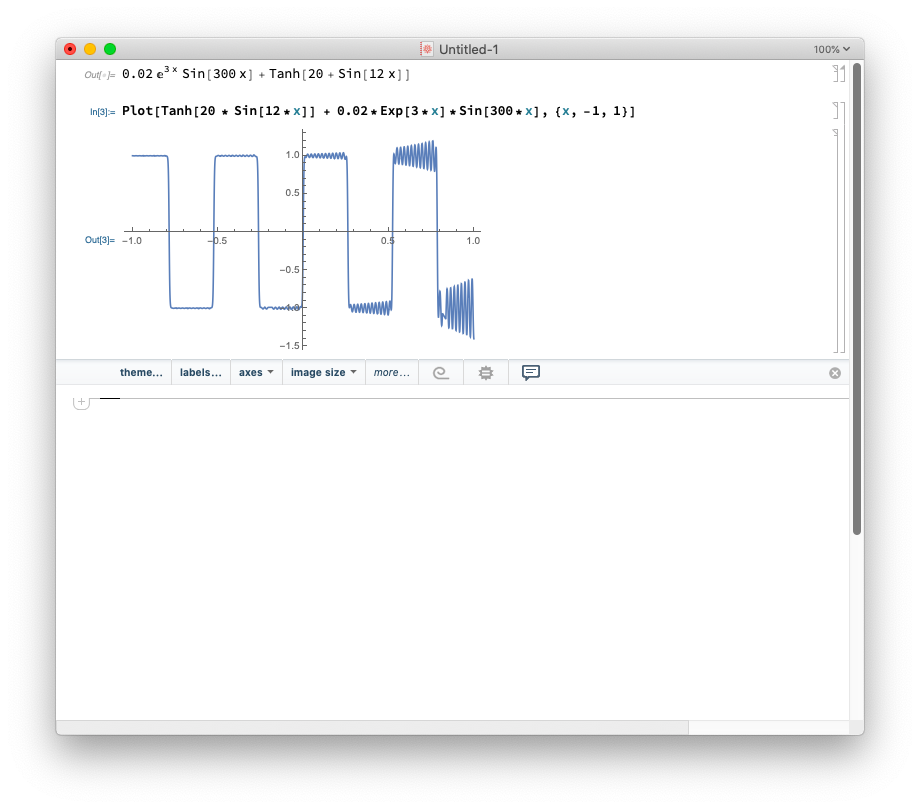
\includegraphics[scale = 0.14]{images/1_1_4_mma.png}
				\caption{Mma绘制的图像}
			\end{minipage}
			\begin{minipage}{13em}
				\centering
				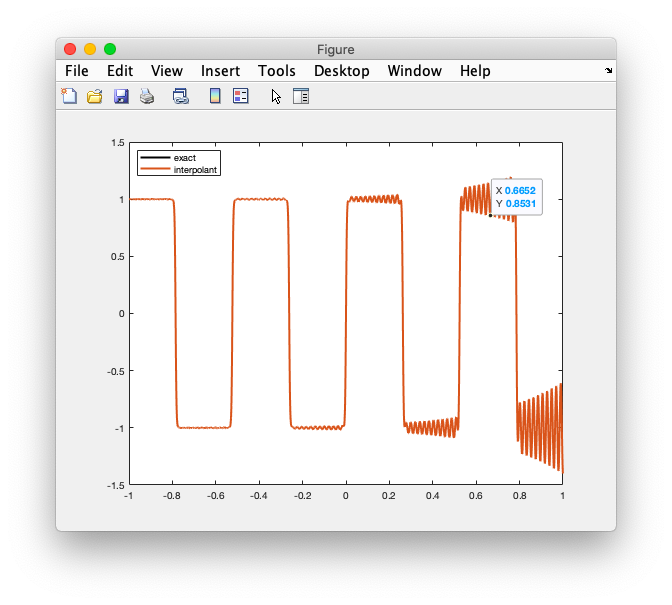
\includegraphics[scale = 0.2]{images/1_1_4_plot.png}
				\caption{被插值函数}
			\end{minipage}
			\begin{minipage}{13em}
				\centering
				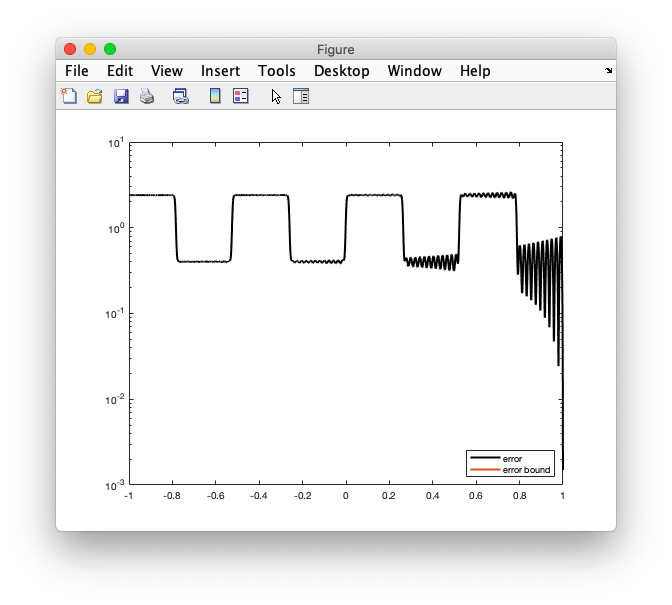
\includegraphics[scale = 0.2]{images/1_1_4_R.png}
				\caption{误差}
			\end{minipage}
		\end{figure}

	\section{三次样条插值}
	\subsection{第一类边值条件}
		在老师给出的三次样条插值代码的基础上,去掉有关作出插值图像的代码,增加样条函数的返回值:在当前$n$的取值下,这$4n$个点中误差的最大值。计算的方法为:在每一个插值区间上,利用\verb|linspace|函数,选取包括两端点在内的6个比较点(因为两个端点的误差必定为0,故不影响对与每一组最大值的判断),记录其中的最大值,并与全局的最大值比较,最终在循环结束时得到最终的最大误差。主函数内维持一个一维向量,保存对应n的值时的最大误差,最终用\verb|loglog|函数绘制出来。\par
		源代码如下:
		\begin{lstlisting}
clear, clc, clf
LW = 'linewidth'; lw = 2;

% 用于保存三种边值条件下对于不同n的最大误差
maxError1 = zeros(7, 1);
maxError2 = zeros(7, 1);
maxError3 = zeros(7, 1);
% 用于画图
kk = linspace(6, 12, 7);
nn = 2.^kk;
% 循环里面的n为1x1的矩阵,而上面的nn为1x7
for k = 6:12
	n = 2^k;
	x = linspace(-1, 1, n + 1)';
	F = @(x)exp(3 .* cos(pi .* x));
	f = F(x);
	%%
	h = diff(x);
	df = diff(f);
	lambda = h(2:n) ./ (h(2:n) + h(1:n - 1));
	d = 6 * (df(2:n) ./ h(2:n) - df(1:n - 1) ./ ...
		h(1:n - 1)) ./ (h(2:n) + h(1:n - 1));
	mu = 1 - lambda;
	%%
	%第一类边界条件
    M0 = 3*pi^2*exp(-3);
	Mn = 3*pi^2*exp(-3);
	A1 = diag(2 * ones(n - 1, 1)) + ...
		diag(lambda(1:n - 2), 1) + ...
		diag(mu(2:n - 1), -1);
	D1 = [d(1) - mu(1) * M0; d(2:n - 2); ...
		d(n - 1) - lambda(n - 1) * Mn];
	M1 = A1 \ D1;
	M1 = [M0; M1; Mn];
	%%
	%第二类边界条件
	m0 = 0;
	mn = 0;
	lambda2 = [1; lambda];
	mu2 = [mu; 1];
	d0 = 6 * (df(1) / h(1) - m0) / h(1);
	dn = 6 * (mn - df(n) / h(n)) / h(n);
	D2 = [d0; d; dn];
	A2 = diag(2 * ones(n + 1, 1)) + ...
		diag(lambda2, 1) + diag(mu2, -1);
	M2 = A2 \ D2;
	%%
	%第三类边界条件
	lambda0 = h(1) / (h(1) + h(n));
	lambda3 = [lambda0; lambda(1:n - 2)];
	mu0 = 1 - lambda0;
	d0 = 6 * (df(1) ./ h(1) - df(n) ...
		./ h(n)) / (h(1) + h(n));
	D3 = [d0; d];
	A3 = diag(2 * ones(n, 1)) + ...
		diag(lambda3, 1) + diag(mu, -1);
	A3(1, n) = mu0;
	A3(n, 1) = lambda(n - 1);
	M3 = A3 \ D3;
	M3 = [M3; M3(1)];
	%%
	% 接收返回值到数组
	maxError1(k - 5) = CubicSpline(x, F, h, M1);
	maxError2(k - 5) = CubicSpline(x, F, h, M2);
	maxError3(k - 5) = CubicSpline(x, F, h, M3);
end
figure(1);
loglog(nn, maxError1), hold on
loglog(nn, maxError2), hold on
loglog(nn, maxError3)
legend('第一类边界条件', '第二类边界条件', ...
	'第三类边界条件', 'location', 'nw')


function maxTestError = CubicSpline(x, F, h, M)
	% LW = 'linewidth'; lw = 2;
	% n = 2^6;
	n = size(x) - 1;
	f = F(x);
	maxTestError = 0;

	for k = 1:n
		% testPoint为一个1x6的数组,借助数组运算保存
		% 一个插值区间中的6个误差
		testPoint = linspace(x(k), x(k + 1), 6)';
		S = ((x(k + 1) - testPoint).^3 * M(k) ...
			+ (testPoint - x(k)).^3 * M(k + 1)) ...
			/ (6 * h(k)) + ((x(k + 1) - testPoint) ...
			* f(k) + (testPoint - x(k)) * f(k + 1)) ...
			/ h(k) - h(k) * ((x(k + 1) - testPoint) * ...
			M(k) + (testPoint - x(k)) * M(k + 1)) / 6;
		testError = abs(F(testPoint) - S);
		maxThisRound = max(testError);
		maxTestError = max(maxTestError, maxThisRound);
	end
end
		\end{lstlisting}
		运行结果如图所示
		\begin{figure}[h!]
			\centering
			\begin{minipage}{20em}
				\centering
				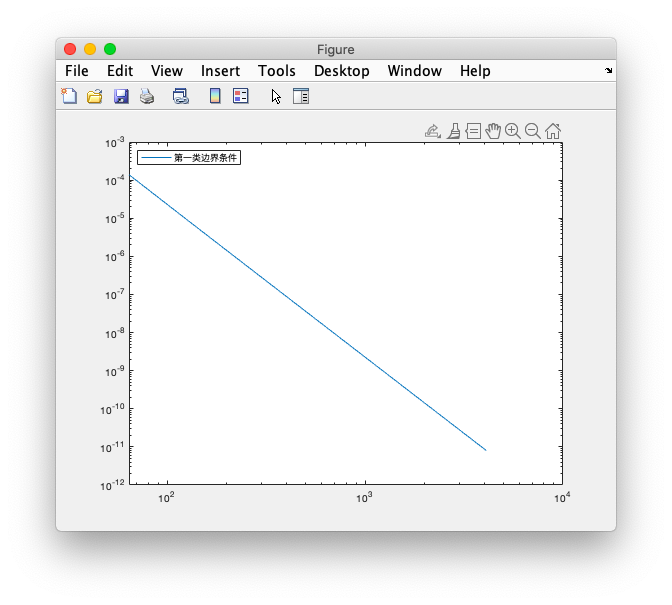
\includegraphics[scale = 0.3]{images/1_2_1.png}
				\caption{2.1题 第一类边值条件}
			\end{minipage}
			\begin{minipage}{20em}
				\centering
				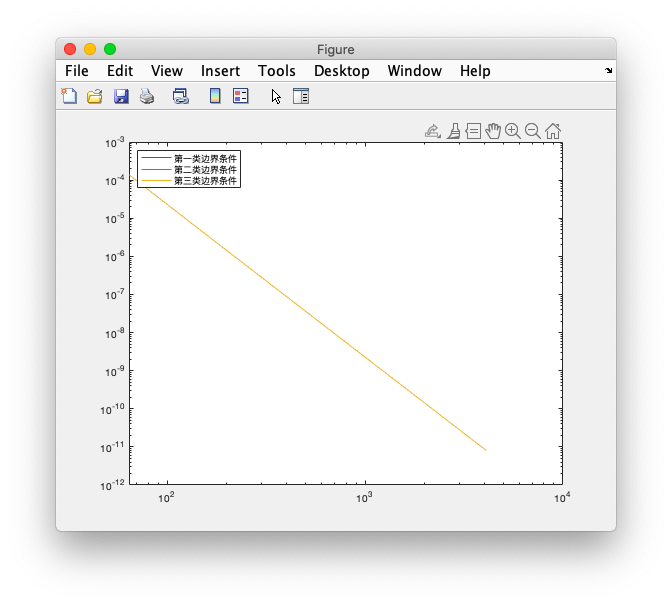
\includegraphics[scale = 0.3]{images/1_2_3.png}
				\caption{2.3题 第一、二、三类边值条件}
			\end{minipage}
		\end{figure}
		\subsection{斜率的含义}
			不妨设n和R满足如下线性关系式
			\[\ln R=\ln a+b\ln n\]
			对等式两边同时取自然指数,得
			\[R=an^b\]
			故\verb|log-log|图的斜率b表示R和n满足b次多项式关系
		\subsection{第二、三类边值条件}
		代码基本思想相同,代码见上文注释为二、三类边值条件的部分

	\section{最小二乘拟合}
		\subsection{最小二乘拟合}
		调用\verb|polyfit|函数只能做多项式拟合,于是将y变量取对数。源代码如下:
		\begin{lstlisting}
clear, clc, clf

x = [-0.70, -0.50, 0.25, 0.75];
y = [0.99, 1.21, 2.57, 4.23];

plot(x, y, 'o'); hold on

z = log(y);
p = polyfit(x, z, 1);
x1=-1:0.01:1;
z1=polyval(p,x1);
y1=exp(z1);
plot(x1,y1,'r');
y1(1,31)
y1(1,51)
y1(1,126)
y1(1,176)
		\end{lstlisting}
		其中最下面的四行用于输出$x=-0.70,-0.50,0.25,0.75$四处的值,用以和原始数据进行比较并计算出2-范数。拟合结果为:\par
		\begin{figure}[h!]
			\centering
			\begin{minipage}{40em}
				\centering
				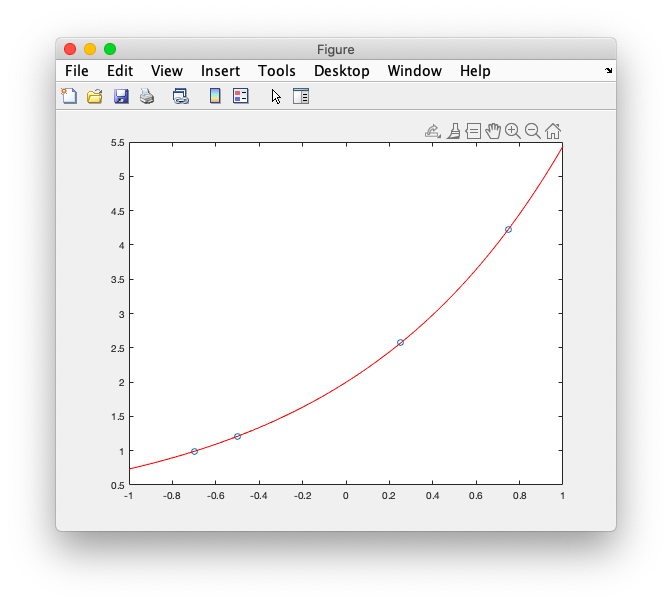
\includegraphics[scale = 0.35]{images/1_3.png}
				\caption{最小二乘指数拟合}
			\end{minipage}
		\end{figure}
		误差的2-范数计算如下:
		\[\begin{aligned}
			\parallel R\parallel_2&=\sqrt{(0.9904-0.99)^2+(1.2102-1.21)^2+(2.5658-2.57)^2+(4.2345-4.23)^2}\\
			&=0.0045265881191
		\end{aligned}\]

\end{document}
